\documentclass[twoside,10pt]{article}
\usepackage{shlists}
\usepackage[utf8]{inputenc}
\usepackage[spanish]{babel}
\usepackage[T1]{fontenc}


\usepackage{multicol}
\usepackage{picinpar}

\usepackage{url}
\newcommand{\surl}[1]{{\small\url{#1}}}

\newcounter{vol}
\newcounter{num}
\newcounter{anyo}
\setcounter{vol}{9}
\setcounter{num}{3}
\setcounter{anyo}{2016}
\newcommand{\mes}{Septiembre}
\usepackage{revisionNLcol}


\title{\ \\ Docencia 2.0\\ \large Juan Julián Merelo, Fernando Tricas}
\author{\LARGE Lenguajes de programación: ¿uno, ninguno o todos?}

\date{}

\AutTit{Docencia 2.0}

\begin{document}
\addtocounter{page}{2}

\maketitle

\vspace*{-5ex}

\begin{multicols}{2}

Si hay un tema transversal en la informática son los lenguajes de
programación. Desde los niveles más bajos de la arquitectura a los más
altos, la forma universal en la que el ser humano se comunica con un
ordenador son los programas, escritos en alguno de los lenguajes de
programación disponibles. Los lenguajes suelen tener una serie de
características comunes: una sintaxis rígida, implementaciones con
licencia libre y una evolución continua.

En esta última característica está uno de los problemas. El lenguaje
que enseñaste en primero puede no parecerse en nada al que usarás en
el trabajo de fin de grado. Pero si consideramos que la evolución
individual está acompañada de una evolución colectiva de los tipos de
lenguajes que se usan y que, por tanto, se necesitan no ya para
conseguir un puesto de trabajo, sino siquiera para poder trabajar en
un entorno de computación determinado, la elección de un lenguaje de
programación para una asignatura o para una carrera entera se convierte en
una tarea ardua o imposible.

Porque, seamos prácticos, elegir un sólo lenguaje para regirlos a
todos es imposible en nuestro país. Ni en ninguno, para el caso.
Nuestra idiosincrasia impediría que más de dos personas se pusieran de
acuerdo en qué lenguaje usar desde primero a cuarto, y en el caso
improbable de que un \emph{ukase} de la superioridad impusiera uno, esa
misma idiosincrasia haría que el profesor de prácticas de tercero usara
eventualmente el que le viniera en gana. 
Seguramente esto es hasta sano y saludable porque, ¿quién nos aseguraría
que en el ``mundo real'' la sociedad y la industria habría elegido este
supuesto lenguaje ganador y tan perfecto para habernos puesto de acuerdo a
nosotros? Habrá que agradecerle al profesor de prácticas de tercero el que
el alumno  haya tenido exposición a diversos lenguajes y
entornos de trabajo. Por esa misma razón descartamos esa opción
del lenguaje único y puro para dominarlos a todos.

También podríamos pensar, siguiendo las metodologías modernas, la idea de
adaptación al estudiante: cada cuál que elija su lenguaje favorito y que lo
utilice
para desarrollar sus proyectos. Seguramente nos encontraríamos con algunas
dificultades: lenguajes poco adecuados para las tareas que están
relacionadas con la temática de la asignatura, excesivo 
``monocultivo'',
dado que es fácil ponerse de acuerdo con uno mismo y terminar haciendo todo
con una sola tecnología (perdiendo en el camino la oportunidad de
explorar otras), y la
no despreciable complejidad de prestar asistencia en caso de que alguna cosa no
vaya bien. 

Desde nuestra experiencia esta puede ser una buena aproximación cuando
vamos avanzando en la carrera: sugerir, por ejemplo, un lenguaje que
nosotros creamos adecuado pero facilitar que se elijan alternativas.
Eventualmente, el profesor no tiene que evaluar al
alumno por la letra de lo que haya hecho, es decir, la literalidad de
haber escrito algún algoritmo o usado una estructura de datos en un
lenguaje que el profesor conoce, sino por el hecho de que haya sido
capaz de entender esos conceptos y usarlos en la práctica. No
resultaría difícil, para cualquier profesor, evaluar la consecución de
los objetivos por parte del alumno en casi cualquier lenguaje de
programación. Salvo, quizá, Haskell.

Vamos avanzando.


%--------------------------
\noindent\rule{86mm}{1pt}
\vspace{1ex} {\small{\begin{window}[0,r,
\includegraphics[width = 27mm]{JJM.jpg},] 
\noindent\emph{JJ Merelo} es catedrático de Universidad
en el área de Arquitectura y Tecnología de Computadores, y
actualmente director de la Oficina de Software Libre de la UGR.
Últimamente le ha dado por el \textsl{flipped
learning}, de lo que se informará debidamente en esta columna.
\end{window}}} 
\medskip

{\small{\begin{window}[0,r,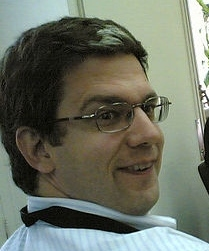
\includegraphics[width = 27 mm]{FTricas1.jpg},]
		\noindent \emph{Fernando Tricas García} es profesor
		titular de Lenguajes y Sistemas Informáticos del Departamento
		de Informática e Ingeniería de Sistemas de la Universidad de
		Zaragoza.  Empezó a estudiar la blogosfera casi cuando aún no
		existía (allá por el año 2002) y a tratar de integrarla en los
		cursos y tareas docentes un poco después.  Ha impartido
		numerosas charlas relacionadas con el tema de la Web 2.0, 
		internet y universidad,\ldots\ 
		Actualmente es Vicerrector de Tecnologías de la Información y
de la Comunicación.   
		\end{window}}}
%-------------------------------------------------

 
¿Y en primero? 

Lo que siempre se dice en estos casos es que se trata de aprender a
programar: las bases, conceptos, la organización de un programa, las
estructuras de datos, entre otros, y que el lenguaje no es lo importante.
Pero luego todo el mundo tiene argumentos para defender unos
y desdeñar otros.

El problema es que, frente a la posibilidad de que el alumno use su
propio lenguaje o usar un sólo lenguaje, nos barruntamos que obligar
al alumno de primero a usar varios diferentes, cada uno con
sus bases, su historia, sus herramientas, no es la mejor opción. 
Realmente no hay lenguaje de programación moderno que no
implemente todos los conceptos que debe aprender un alumno de
primero. El que todas las asignaturas de un primero de Informática u
otra carrera TIC adoptaran un sólo lenguaje permitiría a los profesores
concentrarse en los conceptos en sí y no tener que dedicar una o
varias sesiones de prácticas a las complejidades intrínsecas de
compilar en Java o en Pascal o cómo instalar paquetes en R. Una
encuesta informal en cualquier escuela de informática te permitirá
descubrir que en primero, y muchas veces en el primer cuatrimestre,
diferentes asignaturas usan lenguajes o entornos tan disimilares como
R, Maxima, Java, C++, \mbox{Python} e incluso C, además de algún
que otro lenguaje máquina. Todo ello en primero de carrera, en los
primeros meses, y en aras de \emph{facilitar al alumno la tarea}. 

Nada más lejos de la realidad. El principal obstáculo para la
implantación de \emph{Un Sólo Lenguaje} en primero es la dificultad
en decidir cuál es ese lenguaje. Incluso decidir el tipo, si
funcional, dirigido a objetos, procedural... Sin embargo, no es una
dificultad insalvable y lo único que habría que hacer es decir qué
requisitos deben tener los lenguajes que usan en las diferentes
asignaturas y buscar el que más acomode todos esos requisitos. 
Un problema informático, con una solución informática relativamente
simple. Y si es imposible encontrar ese lenguaje único, dos o tres
lenguajes, quizás a diferente nivel de la arquitectura de un
ordenador, son mejor solución que una multiplicidad de lenguajes,
algunos con escaso recorrido a lo largo de la carrera.

Imaginad que los alumnos llegaran a segundo controlando bien, con cierta
eficacia, un lenguaje, uno sólo. Eso permitiría, a partir de ahí,
dejarle libertad para que elija nuevos lenguajes en asignaturas, como
las que se dan en segundo, que no están, en general, enfocadas a un
lenguaje específico. Usar lenguajes que tengan recorrido en varias
asignaturas va a redundar en un mejor conocimiento por parte del alumno y
dejar libertad, en cursos superiores, para elegir el lenguaje en el
que se implementen los conceptos llevará también a que el alumno
entienda que se confía que sea capaz de elegir el lenguaje más
adecuado para cada tarea y evaluar su desempeño. Una situación que
permitirá que nuestros estudiantes se involucren más en su aprendizaje
de manera proactiva, frente a una situación, a nuestro entender no
deseable, de multiplicidad de lenguajes que no dejan al alumno posibilidad
de elección.

Pensemos, pues, en las bondades de la Gran Unificación de Lenguajes en
la carrera de informática, al menos en el primer y quizás el segundo
semestre. 
Aunque sobre los méritos de algunos lenguajes específicos hablaremos
próximamente en otra columna. 

\noindent  
\bigskip

\noindent\emph{Todas las columnas de la serie Docencia 2.0
pueden descargarse en formato LaTeX desde
\surl{https://github.com/ReVision-Docencia-20/Columnas}}

\noindent\rule{90mm}{1pt}

{\small \noindent\copyright 2016 JJ. Merelo, F. Tricas. Este artículo es de acceso libre distribuido bajo los t\'{e}rminos
de la Licencia Creative Commons de Atribuci\'{o}n, que permite copiar,
distribuir y comunicar p\'{u}blicamente la obra en cualquier medio, s\'{o}lido
o electr\'{o}nico, siempre que se acrediten a los autores y fuentes
originales}

\end{multicols}
\end{document}